\documentclass[a4paper,fleqn,12pt]{article}
\usepackage[utf8]{inputenc}
\usepackage{amsmath}
\usepackage{amssymb}
\usepackage{booktabs}
\usepackage{fancyhdr}
\usepackage{amsthm}
\usepackage{graphicx}
\usepackage{pdfpages}

\begin{document}
\begin{titlepage}
	\setlength{\parindent}{0pt}
	\large
\centering
Techincal University - Sofia \par
Faculty of Applied Mathematics and Informatics \par
\vspace{2cm}

{\huge Project 1 - Topics of Algebra\par}

\vspace{2cm}

\vspace{1cm}
{\LARGE\scshape  Solution for version 4 \par}



\vfill

\begin{minipage}[t]{.5\linewidth}
	Student: \\
	Kristian Krachmarov \\
	791324005
\end{minipage}%
\begin{minipage}[t]{.5\linewidth}
	\raggedleft
	Examiner:\\
	Prof. Mirko Tarulli
\end{minipage}

\vspace{2cm}
\raggedright

\end{titlepage}
\pagenumbering{gobble}
\tableofcontents
\newpage
%\fontsize{14pt}{16pt}\selectfont
\pagenumbering{arabic}
\newpage

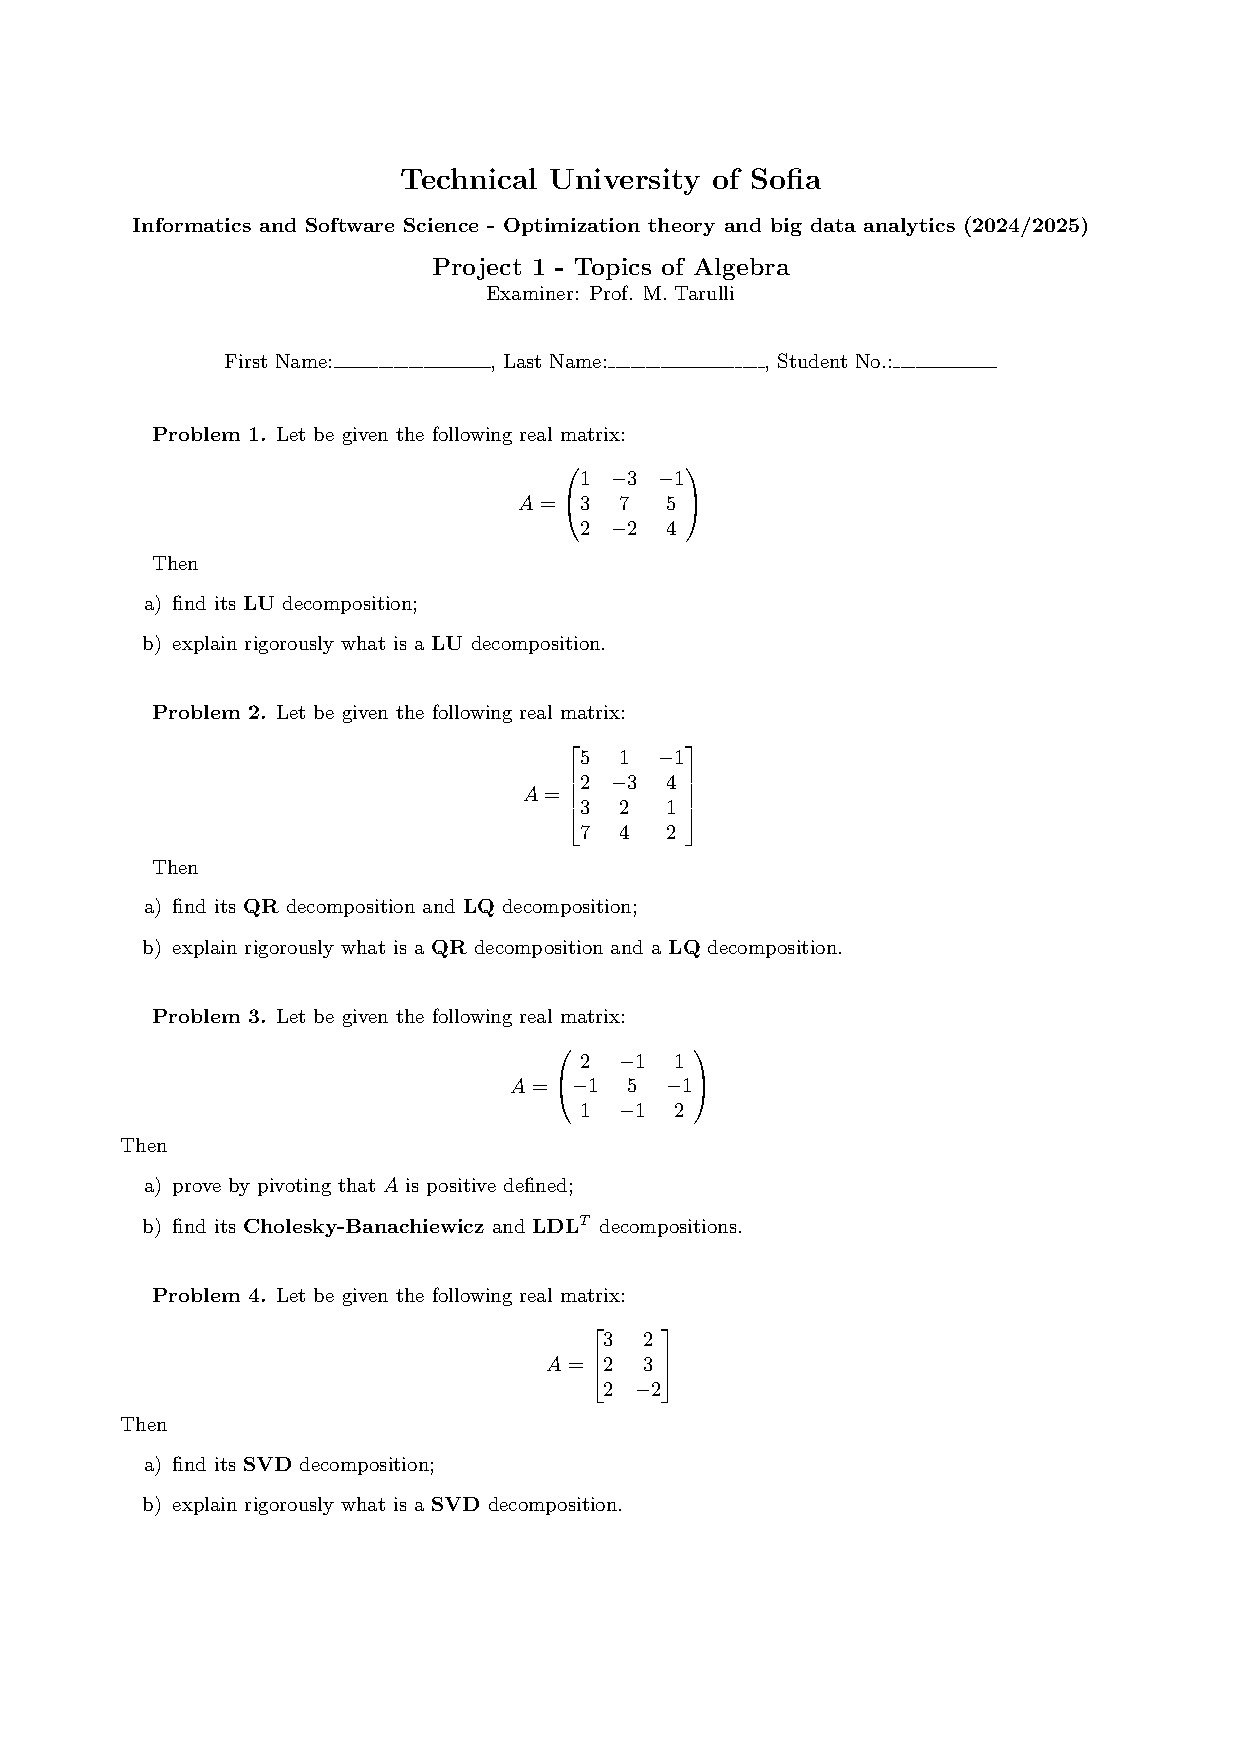
\includepdf[pages=-]{Project1-Version4-2425.pdf}
\newpage

\section{Problem 1}
$$ A = 
	\begin{pmatrix}
	1 & -3 & -1 \\
	3 & 7 & 5 \\
	2 & -2 & 4 \\
	\end{pmatrix}
$$
\subsection{Solution for 1a}
Lets start with L being the identity matrix
$$
	L = \begin{pmatrix}
	1 & 0 & 0 \\
	0 & 1 & 0 \\
	0 & 0 & 1 \\
	\end{pmatrix}
$$
We perform the following operations on matrix A: 
$$
\begin{array}{|l@{}}
	R_2 = R_2 - 3R_1 \\
	R_3 = R_3 - 2R_1
\end{array}
$$
Where $R_i$ is the $i$th row of the matrix. \\
We write the coefficient 3 in the matrix L at row 2 and column 1. 
The same can be done for the coefficient 2 for row 3 and column 1.
$$
	L = \begin{pmatrix}
	1 & 0 & 0 \\
	3 & 1 & 0 \\
	2 & 0 & 1 \\
	\end{pmatrix} \qquad 
	A = \begin{pmatrix}
	1 & -3 & -1 \\
	0 & 16 & 8 \\
	0 & 4  & 6 \\
	\end{pmatrix}
$$
We perform the following operation on matrix A
$$
R_3 = -\frac{1}{4}R_2 + R_3
$$
We write the coefficient $\frac{1}{4}$ in matrix L at row 3 and column 2.
$$
L = \begin{pmatrix}
	1 & 0 & 0 \\
	3 & 1 & 0 \\
	2 & \frac{1}{4} & 1 \\
	\end{pmatrix} \qquad 
	A = \begin{pmatrix}
	1 & -3 & -1 \\
	0 & 16 & 8 \\
	0 & 0  & 4 \\
	\end{pmatrix} = U
$$
\newpage
\subsection{Solution for 1b}
LU decomposition is a technique for factorizing a square matrix A as a product of two other matrices. 
$$
A = LU
$$
where L is a lower triangular matrix and U is upper triangular matrix. \\
To have LU decomposition the matrix A must be square matrix ($m \times m$ dimensions) and invertible ($A^{-1}$ exists).  \\
The algorithm used to solve this particular matrix is LU without pivoting. 
In this algorithm we initialize L to be identity matrix and we modify A to be an upper triangular matrix like U by performing row operations to create zeroes below the diagonal for each column. Then each multiplier/coefficient is recorded in L for the coresponding row and column. \\
The most common use for LU decomposition is to solve system of linear equations. 
$$
Ax = b 
$$
For the system we can substitute $A = LU$ and we can let $y = Ux$. Then the system becomes $Ly = b$ and after solving it we can solve the other system $Ux = y$

\newpage

\section{Problem 2}
$$
A = \begin{bmatrix}
	5 & 1 & -1 \\
	2 & -3 & 4 \\
	3 & 2 & 1 \\
	7 & 4 & 2 \\
\end{bmatrix}
$$
\subsection{Solution for 2a}
First we perform the Grand-Schmidt process for each column of the matrix
$$
v_1 = \begin{bmatrix} 5 \\ 2 \\ 3 \\ 7   \end{bmatrix} \quad
v_2 = \begin{bmatrix} 1 \\ -3 \\2 \\ 4  \end{bmatrix} \quad
v_3 = \begin{bmatrix} -1\\ 4 \\ 1 \\ 2   \end{bmatrix}
$$
We determine the orthogonal vectors $e_k$ by the following formula
$$
e_k = \frac{u_k}{|| u_k ||} \text{ where } \quad u_k = v_k - \sum_{j=1} ^{k} proj_{u_j} v_k \quad ||u_k||  =  \sqrt{\sum_{j=1} ^n  |u_i|^2} \quad proj_a(b) = \frac{a \cdot b}{a \cdot a}a
$$
We solve for each column
\begin{gather*}
u_1 = v_1 = \begin{bmatrix} 5 \\ 2 \\ 3 \\ 7   \end{bmatrix} \implies
e_1 = \frac{u_1}{|| u_1 ||} =
\frac{u_1}{\sqrt{5^2 + 2^2 + 3^2 + 7^2}} =
 \frac{u_1}{\sqrt{87}} = \begin{bmatrix} \frac{5\sqrt{87}}{87} \\ \frac{2\sqrt{87}}{87} \\ \frac{3\sqrt{87}}{87} \\ \frac{7\sqrt{87}}{87}   \end{bmatrix} \approx 
\begin{bmatrix} 0.54 \\ 0.21 \\ 0.32 \\ 0.75   \end{bmatrix} \\
 \\
u_2 = v_2 - proj_{u_1} (v_2) = v_2 - \frac{u_1 \cdot v_2}{ u_1 \cdot u_1}u_1 = v_2 - \frac{(1 \cdot 5) + (-3) \cdot 2 + (2 \cdot 3) + (4 \cdot 7)}{\sqrt{87}^2} u_1 = \\
u_2 = v_2 - \frac{33}{87} u_1 = v_2 - \frac{11}{29} u_1 = \begin{bmatrix} 1 \\ -3 \\2 \\ 4  \end{bmatrix} - \frac{11}{29} \begin{bmatrix} 5 \\ 2 \\ 3 \\ 7   \end{bmatrix} = \begin{bmatrix} 1 - \frac{55}{29} \\ -3 - \frac{22}{29} \\2 - \frac{33}{29} \\ 4 - \frac{77}{29} \end{bmatrix} =
\begin{bmatrix} -\frac{26}{29} \\ -\frac{109}{29} \\\frac{25}{29} \\ \frac{39}{29}  \end{bmatrix} \approx \begin{bmatrix} -0.90 \\ -3.76 \\ 0.86 \\ 0.75  \end{bmatrix} \\
e_2 = \frac{u_2}{|| u_2 ||} = \frac{u_2}{\sqrt{-0.9^2 + -3.76^2 + 0.86^2 + 1.34^2}} =
 \frac{u_2}{\sqrt{17.48}} \approx \begin{bmatrix} -0.21\\ -0.90 \\ 0.21 \\ 0.32   \end{bmatrix} \\
\end{gather*}
\begin{gather*}
u_3 = v_3 - proj_{u_1} (v_3) - proj_{u_2} (v_3) = v_3 -  \frac{u_1 \cdot v_3}{ u_1 \cdot u_1}u_1 -  \frac{u_2 \cdot v_3}{ u_2 \cdot u_2}u_2 \\
\frac{u_1 \cdot v_3}{ u_1 \cdot u_1}u_1 = \frac{-5 + (4\cdot2) + (1\cdot 3) +( 2 \cdot 7)}{\sqrt{87}^2} u_1 = \frac{20}{87}  \begin{bmatrix} 5 \\ 2 \\ 3 \\ 7   \end{bmatrix} =  
 \begin{bmatrix} 1.14 \\ 0.46 \\ 0.69 \\ 1.61  \end{bmatrix} \\
\frac{u_2 \cdot v_3}{ u_2 \cdot u_2}u_2 = \frac{0.9 + (-3.76 \cdot 4) + 0.86 + (0.75 \cdot 2)}{17.48}u_2 = \frac{-11.78}{17.48}u_2 = 
\begin{bmatrix} 0.65 \\ 2.72 \\ -0.62 \\ -0.54   \end{bmatrix}\\
u_3 = \begin{bmatrix} -1\\ 4 \\ 1 \\ 2 \end{bmatrix} - \begin{bmatrix} 1.14 \\ 0.46 \\ 0.69 \\ 1.61  \end{bmatrix}  - \begin{bmatrix} 0.65 \\ 2.72 \\ -0.62 \\ -0.54   \end{bmatrix} = 
\begin{bmatrix}- 2.69 \\ 1.26 \\ 0.83 \\1.21   \end{bmatrix} \\
e_3 = \frac{u_3}{|| u_3 ||} = \frac{u_3}{\sqrt{-2.69^2 + 1.26^2 + 0.83^2 + 1.21^2}}= \frac{u_3}{\sqrt{10.99}} = \begin{bmatrix} - 0.81 \\ 0.38 \\ 0.25 \\ 0.36  \end{bmatrix}
\end{gather*}
After we create the orthogonal basis we can create the Q matrix.
$$
Q = 
\begin{pmatrix} 
0.54 & -0.21 & -0.81 \\
0.21 & -0.90 & 0.38 \\
0.32 & 0.21 & 0.25 \\
0.75 & 0.32 & 0.36
\end{pmatrix}
$$
We can find R by the following formula 
$$
R = Q^T A
$$
$$
Q^T = 
\begin{pmatrix} 
0.54 & 0.21 & 0.32 & 0.75 \\
-0.21 & -0.9 & 0.21 & 0.32 \\
-0.81 & 0.38 & 0.25 & 0.36 \\
\end{pmatrix}
$$
$$
Q^TA =
 \begin{pmatrix} 
0.54 & 0.21 & 0.32 & 0.75 \\
-0.21 & -0.9 & 0.21 & 0.32 \\
-0.81 & 0.38 & 0.25 & 0.36 \\
\end{pmatrix} 
\begin{bmatrix}
	5 & 1 & -1 \\
	2 & -3 & 4 \\
	3 & 2 & 1 \\
	7 & 4 & 2 \\
\end{bmatrix} = 
\begin{pmatrix}
9.33 & 3.54 & 2.14 \\
0 & 4.18 & -2.53 \\
0 & 0 & 3.31
\end{pmatrix} = R
$$
We can find $L$ by transposing $R$.
$$
L = R^T = 
\begin{pmatrix}
9.33 & 0 & 0 \\
3.54 & 4.18 & 0 \\
2.14 & -2.53 & 3.31 \\
\end{pmatrix} 
$$

\newpage
\subsection{Solution for 2b}
\newpage

\section{Problem 3}
$$
A = 
\begin{pmatrix}
2 & -1 & 1 \\
-1 & 5 & -1 \\
1 & -1 & 2 
\end{pmatrix}
$$
\subsection{Solution for 3a}
To prove that A is positive defined by pivoting we will transform the matrix into an upper triangular matrix and check if every pivot is positive. The first pivot is $a_{11} = 2$. Then we perform the following operations on matrix A: 
$$
\begin{array}{|l@{}}
	R_2 = R_2 + \frac{R_1}{2} \\
	R_3 = R_3 - \frac{R_1}{2}
\end{array}
$$
$$
A = \begin{pmatrix}
2 & -1 & 1 \\
0 & \frac{9}{2} & -\frac{1}{2} \\
0 & -\frac{1}{2} & \frac{3}{2} \\
\end{pmatrix}
$$
The next pivot is $a_{22} = \frac{9}{2}$. We perform the following operation
$$
R_3 = R3 - \left(\frac{-\frac{1}{2}}{\frac{9}{2}}\right)R2 = R_3 + \frac{1}{9} R_2
$$
$$
A = \begin{pmatrix}
2 & -1 & 1 \\
0 & \frac{9}{2} & -\frac{1}{2} \\
0 & 0 & \frac{13}{9} \\
\end{pmatrix}
$$
The pivots are $\left( 2, \frac{9}{2}, \frac{13}{9} \right)$ which are all positive numbers.
\newpage
\subsection{Solution for 3b}
The Cholesky decomposition is decomposing the matrix in the form 
$$
A = L \cdot L^T
$$
where L is lower triangular matrix, where each element is calculated by the following formulas
\begin{gather*}
l_{11} = \sqrt{a_{11}}   \\
l_{j1} = \frac{a_{j1}}{l_{11}} \quad  j \in [2, n] \\
l_{ii} = \sqrt{a_{ii} - \sum_{k=1} ^{i-1} l_{ik}} \quad i \in [2, n] \\
l_{ji} = \frac{ \left( a_{ij} - \sum_{k=1} ^{i-1} l_{ik} l_{jk} \right)}{l_{ii}} \quad i \in [2, n-1], j \in [i+1, n] \\
\\
l_{11} = \sqrt{2} = 1.41 \\
l_{21} = \frac{-1}{1.41} = - 0.70 \\
l_{31} = \frac{1}{1.41}  = 0.70 \\
l_{22} = \sqrt{a_{22} - l_{21} ^2} = \sqrt{5 - (-0.70)^2} = \sqrt{4.5} = 2.12 \\
l_{32} = \frac{a_{32} - l_{32}l_{31}}{l_{22}} = \frac{-1 -(0.7)(-0.7)}{2.12} = -0.24 \\
l_{33} = \sqrt{a_{33} - (l_{31} ^2 + l_{32} ^2)} = \sqrt{2 - (0.7^2 + (-0.24^2))} = 1.20\\
\\
L = 
\begin{pmatrix}
1.41 & 0 & 0 \\
-0.70 & 2.12 & 0 \\
0.70 & -0.24 & 1.20 
\end{pmatrix} \implies  
L^T = \begin{pmatrix}
1.41 & -0.70 & 0.70 \\
0 & 2.12 & -0.23 \\
0 & 0 & 1.20
\end{pmatrix}
\end{gather*}
\newpage
To find the $LDL^T$ decomposition we need to find the two matrices: $L$ and $D$.
L is a lower triangular matrix and D is a diagonal matrix.
We can find each element with the following formulas
$$
d_{ii} = a_{ii} - \sum_{j=1} ^{i-1} l_{ij} ^2 \cdot d_{jj} \qquad
l_{ii} = \frac{1}{d_{ii}} \left( a_{ij} - \sum_{k=1} ^{i-1} l_{ik}\cdot l_{jk}\cdot d_{kk} \right)  
$$
\begin{gather*}
L = \begin{pmatrix}
1 & 0 & 0 \\
l_{21}& 1& 0 \\
l_{31} & l_{32} & 1
\end{pmatrix} \qquad 
D = \begin{pmatrix}
d_{11} & 0 & 0 \\
0 & d_{22} & 0 \\
0 & 0 & d_{33}
\end{pmatrix} \\ \\
d_{11} = a_{11} = 2 \\
l_{21} = \frac{1}{d_{11}} \left( a_{21} - \sum_{k=1} ^0 l_{2k}l_{1k}d_{kk} \right) = \frac{1}{2} (-1) = -0.5 \\
l_{31} = \frac{1}{d_{11}} \left( a_{31} - \sum_{k=1} ^0 l_{2k}l_{1k}d_{kk} \right) = \frac{1}{2} (1) = 0.5 \\
\\
d_{22} = a_{22} - \sum_{k=1} ^1 l_{2k} ^2 d_{kk} = 5 - (l_{21} ^2 \cdot d_{11} ) = 5 - (0.5^2 \cdot 2 ) = 5-0.5 = 4.5 \\ 
l_{32} = \frac{1}{d_{22}} \left( a_{32} - \sum_{k=1} ^1 l_{3k}l_{2k}d_{kk} \right) = \frac{1}{4.5} \left(-1 - (l_{31}\cdot l_{21}\cdot d_{11} \right) = \\
\frac{1}{4.5} (-1 -(0.5\cdot (-0.5) \cdot 2)) = \frac{1}{4.5} (-1 + 0.5) = \frac{1}{4.5} \cdot (-0.5) \approx -0.111 \\
\\
d_{33} = a_{33} - \sum_{k=1} ^2 l_{3k} ^2 d_{kk} = 2 - (l_{31} ^2 d_{11} + l_{32} ^2 d_{22}) = 2 - (2 \cdot 0.5^2 + 4.5 \cdot (-0.111)^2 ) \approx 1.444 \\
\\
L = \begin{pmatrix}
1 & 0 & 0 \\
-0.5& 1& 0 \\
0.5 &-0.111 & 1
\end{pmatrix} \quad 
D = \begin{pmatrix}
2 & 0 & 0 \\
0 & 4.5 & 0 \\
0 & 0 & 1.444
\end{pmatrix} \quad 
L^T = \begin{pmatrix}
1 & -0.5 & 0.5 \\
0 & 1& -0.111\\ 
0 &0 & 1
\end{pmatrix} 
\end{gather*}
\newpage

\section{Problem 4}
$$
A = \begin{bmatrix}
3 & 2 \\
2 & 3 \\
2 & -2 \\
\end{bmatrix}
$$
\subsection{Solution for 4a}
To find the Singular Value Decomposition or SVD we need to construct the matrises $U, S, V$. To do that we need to create $A^T$.
$$
A^T = \begin{bmatrix}
3 & 2 & 2 \\
2 & 3 & -2
\end{bmatrix}
$$
We calculate $W = A^T A$
$$
W = 
\begin{bmatrix}
3 & 2 & 2 \\
2 & 3 & -2
\end{bmatrix} \cdot
\begin{bmatrix}
3 & 2 \\
2 & 3 \\
2 & -2 \\
\end{bmatrix} 
 = 
\begin{bmatrix}
17 & 8 \\
8 & 17
\end{bmatrix}
$$
Next we need to find the eigenvalues and eigenvectors. To find the eigenvalues we need to calculate 
$$\det (W -\lambda I) = 0$$
\begin{gather*}
\det (W - \lambda I) = 0 \implies 
\begin{vmatrix}
17-\lambda & 8 \\
8 & 17-\lambda 
\end{vmatrix} = 0 \\
(17-\lambda)^2 - 8^2 = 0 \\
(17-\lambda + 8)(17-\lambda -8) = 0 \\
(25 - \lambda) (9-\lambda)= 0 \\
\lambda_1 = 25 \qquad \lambda_2 = 9 
\end{gather*}
To find the eigenvectors we need to calculate for each eigenvalue the following expression
$$
(W - \lambda I ) X = 0
$$
where $X = (x_1, x_2)^T$
\begin{gather*}
\lambda_1 = 25 \implies 
\begin{pmatrix}
17-25 & 8 \\
8 & 17-25
\end{pmatrix} \cdot  
\begin{pmatrix} x_1 \\ x_2 \end{pmatrix} = 
\begin{pmatrix}
-8 & 8 \\
8 & -8
\end{pmatrix}\cdot  
\begin{pmatrix} x_1 \\ x_2 \end{pmatrix} = 0 \\
-8x_1 + 8x_2 = 0 \implies x_1 = x_2 \implies v =  \begin{bmatrix} 1 \\1 \end{bmatrix}  \\
|| v || = \sqrt{1^2 + 1^2} = \sqrt{2} \implies v_1 = \frac{1}{\sqrt{2}} \begin{bmatrix} 1 \\1 \end{bmatrix} 
\end{gather*}
\begin{gather*}
\lambda_2 = 9 \implies 
\begin{pmatrix}
17-9 & 8 \\
8 & 17-9
\end{pmatrix} \cdot  
\begin{pmatrix} x_1 \\ x_2 \end{pmatrix} = 
\begin{pmatrix}
8 & 8 \\
8 & 8
\end{pmatrix}\cdot  
\begin{pmatrix} x_1 \\ x_2 \end{pmatrix} = 0 \\
8x_1 + 8x_2 = 0 \implies x_1 = -x_2 \implies v =  \begin{bmatrix} 1 \\-1 \end{bmatrix} \\
|| v || = \sqrt{1^2 + (-1)^2} = \sqrt{2}  \implies v_2 = \frac{1}{\sqrt{2}} \begin{bmatrix} 1 \\-1 \end{bmatrix} 
\end{gather*}
Using $v_1, v_2$ we can create the matrix $V$
$$
V = 
\begin{bmatrix} 
\frac{1}{\sqrt{2}} & \frac{1}{\sqrt{2}} \\
\frac{1}{\sqrt{2}} & -\frac{1}{\sqrt{2}}
\end{bmatrix}
$$
To get the $S$ matrix we need to calculate the singular values, which are the square root of each nonzero eigenvalue
$$
\sigma_1 = 5 \qquad \sigma_2 = 3 \implies
S = 
\begin{bmatrix}
5 & 0 \\
0 & 3 \\
0 & 0
\end{bmatrix}
$$
To construct $U$ we need to calculate $u_1 = \frac{Av_1}{\sigma_1}$ and $u_2 = \frac{Av_2}{\sigma_2}$
\begin{gather*}
Av_1 =
\begin{bmatrix}
3 & 2 \\
2 & 3 \\
2 & -2 \\
\end{bmatrix} \cdot 
\frac{1}{\sqrt{2}} \begin{bmatrix} 1 \\1 \end{bmatrix}  = \frac{1}{\sqrt{2}} \begin{bmatrix} 5 \\ 5 \\0 \end{bmatrix} =  \begin{bmatrix} \frac{5}{\sqrt{2}} \\ \frac{5}{\sqrt{2}} \\0 \end{bmatrix} \\
 u_1 = \frac{Av_1}{\sigma_1} = \frac{1}{5} \begin{bmatrix} \frac{5}{\sqrt{2}} \\ \frac{5}{\sqrt{2}} \\0 \end{bmatrix} = 
\begin{bmatrix} \frac{\sqrt{2}}{2}  \\ \frac{\sqrt{2}}{2}  \\0 \end{bmatrix} \\
\\
Av_2  = \begin{bmatrix}
3 & 2 \\
2 & 3 \\
2 & -2 \\
\end{bmatrix} \cdot 
\frac{1}{\sqrt{2}} \begin{bmatrix} 1 \\-1 \end{bmatrix} = \frac{1}{\sqrt{2}} \begin{bmatrix} 1 \\ -1 \\ 4 \end{bmatrix} = 
\begin{bmatrix} \frac{1}{\sqrt{2}} \\ -\frac{1}{\sqrt{2}}\\ \frac{4}{\sqrt{2}} \end{bmatrix} \\
u_2 = \frac{Av_2}{\sigma_2} = \frac{1}{3} \begin{bmatrix} \frac{1}{\sqrt{2}} \\ -\frac{1}{\sqrt{2}}\\ \frac{4}{\sqrt{2}} \end{bmatrix} = 
\begin{bmatrix} \frac{\sqrt{2}}{6} \\ -\frac{\sqrt{2}}{6}\\ \frac{2\sqrt{2}}{3} \end{bmatrix}
\end{gather*}
To calculate $u_3$ we need to find a vector which makes an orthonormal basis for $\mathbb{R}^3$ with $u_1, u_2$ and is a unit vector. To do that we need to solve the following system
\begin{gather*}
\begin{array}{|l@{}}
	\frac{\sqrt{2}}{2}x + \frac{\sqrt{2}}{2}y + 0z = 0 \qquad \qquad | \cdot \frac{2}{\sqrt{2}}  \\
	\frac{\sqrt{2}}{6}x - \frac{\sqrt{2}}{6}y + \frac{2\sqrt{2}}{3}z = 0  \qquad \qquad | \cdot \frac{6}{\sqrt{2}} 
\end{array} \\
\begin{array}{|l@{}}
	x + y + 0z = 0  \qquad \qquad  | R_2 = R_2 + -(R_1)  \\ 
	x - y +4z = 0 
\end{array} \\
-2y + 4z = 0 \implies  y = 2z \\
x = -y = -2z \\
u_3 = \begin{bmatrix} -2z \\ 2z \\z \end{bmatrix} = \begin{bmatrix} -2 \\ 2 \\1 \end{bmatrix} \\
\text{We need to find the unit vector} \\
||u_3|| = \sqrt{(-2)^2 + 2^2 + 1^2} = \sqrt{9} = 3 \implies u_3 = \begin{bmatrix} - \frac{2}{3} \\ \frac{2}{3} \\ \frac{1}{3} \end{bmatrix} 
\end{gather*}
We can build U using $u_1, u_2, u_3$
$$
U = \begin{pmatrix} 
\frac{\sqrt{2}}{2} & \frac{\sqrt{2}}{6} &  -\frac{2}{3}\\
\frac{\sqrt{2}}{2}& -\frac{\sqrt{2}}{2} &  \frac{2}{3}\\
0 & \frac{2\sqrt{2}}{3} & \frac{1}{3}
\end{pmatrix}
$$

\newpage
\subsection{Solution for 4b}


















































\end{document}